% ============================================================
% DA7016: Auto-Assessment System
% Interim Course Project Report
% ============================================================

\documentclass[11pt,a4paper]{article}

\usepackage[
    a4paper,
    top=25mm,
    bottom=25mm,
    left=27mm,
    right=27mm,
    headheight=15pt
]{geometry}

\usepackage[T1]{fontenc}
\usepackage[utf8]{inputenc}
\usepackage{lmodern}
\usepackage{microtype}

\setlength{\parindent}{0pt}
\setlength{\parskip}{6pt}

\usepackage{xcolor}

\definecolor{IITMBlue}{HTML}{1A3C6E}
\definecolor{IITMLightBlue}{HTML}{E8F0FA}
\definecolor{IITMAccent}{HTML}{2B7AB5}
\definecolor{DarkText}{HTML}{1E2328}
\definecolor{MutedText}{HTML}{5C6975}
\definecolor{LightGray}{HTML}{F3F5F8}
\definecolor{MediumGray}{HTML}{D5DAE0}
\definecolor{SuccessGreen}{HTML}{1E7A4D}
\definecolor{WarningAmber}{HTML}{B8751C}

\usepackage{amsmath}
\usepackage{amssymb}
\usepackage{booktabs}
\usepackage{array}
\usepackage{tabularx}
\usepackage{multirow}
\usepackage{makecell}
\usepackage{ragged2e}

\usepackage{graphicx}
\usepackage{tikz}
\usetikzlibrary{positioning,shapes.geometric,arrows.meta,calc,fit}

\usepackage[most]{tcolorbox}
\usepackage{enumitem}

\setlist[itemize]{leftmargin=1.5em, itemsep=3pt, topsep=3pt}
\setlist[enumerate]{leftmargin=1.7em, itemsep=4pt, topsep=3pt}

\usepackage{fancyhdr}
\pagestyle{fancy}
\fancyhf{}
\fancyhead[L]{\small\textcolor{MutedText}{DA7016 --- Auto-Assessment System}}
\fancyhead[R]{\small\textcolor{MutedText}{Interim Course Project Report}}
\fancyfoot[C]{\small\textcolor{MutedText}{\thepage}}
\renewcommand{\headrulewidth}{0.4pt}
\renewcommand{\footrulewidth}{0pt}

\usepackage{titlesec}
\titleformat{\section}{\Large\bfseries\color{IITMBlue}}{\thesection}{0.8em}{}[\vspace{2pt}\color{IITMAccent}\titlerule]
\titleformat{\subsection}{\large\bfseries\color{DarkText}}{\thesubsection}{0.7em}{}
\titleformat{\subsubsection}{\normalsize\bfseries\color{IITMBlue}}{\thesubsubsection}{0.6em}{}
\titlespacing*{\section}{0pt}{22pt}{10pt}
\titlespacing*{\subsection}{0pt}{16pt}{6pt}
\titlespacing*{\subsubsection}{0pt}{12pt}{4pt}

\usepackage[font=small,labelfont={bf,color=IITMBlue},textfont={color=MutedText},labelsep=period]{caption}
\usepackage[colorlinks=true,linkcolor=IITMBlue,citecolor=IITMAccent,urlcolor=IITMAccent]{hyperref}
\usepackage[nameinlink,noabbrev]{cleveref}

\usepackage[backend=biber,style=numeric-comp,sorting=none,maxbibnames=6]{biblatex}
\addbibresource{references.bib}

\newtcolorbox{keyfinding}{
    enhanced, breakable,
    colback=IITMLightBlue, colframe=IITMBlue,
    boxrule=0.8pt, arc=2mm,
    left=5mm, right=5mm, top=4mm, bottom=4mm,
    fontupper=\small, before skip=8pt, after skip=10pt
}

\newtcolorbox{recommendation}{
    enhanced, breakable,
    colback=white, colframe=SuccessGreen,
    boxrule=1pt, borderline west={3pt}{0pt}{SuccessGreen},
    arc=1mm, left=5mm, right=5mm, top=4mm, bottom=4mm,
    fontupper=\small, before skip=8pt, after skip=10pt
}

\newtcolorbox{caveat}{
    enhanced, breakable,
    colback=LightGray, colframe=MediumGray,
    boxrule=0.6pt, arc=1mm,
    left=5mm, right=5mm, top=3mm, bottom=3mm,
    fontupper=\small, before skip=8pt, after skip=10pt
}

\newcommand{\BodhanAI}{\textsc{Bodhan.AI}}
\newcommand{\OpenRouter}{\textsc{OpenRouter}}

\begin{document}

\begin{titlepage}
    \thispagestyle{empty}
    \begin{flushleft}
        \textcolor{IITMAccent}{\rule{0.18\textwidth}{3pt}}
    \end{flushleft}
    \vspace{0.8cm}
    {\Large \textcolor{IITMBlue}{\textbf{Department of Data Science and Artificial Intelligence}}} \\[0.25cm]
    {\normalsize \textcolor{MutedText}{Indian Institute of Technology Madras}}
    \vfill
    {\Huge \color{IITMBlue} \textbf{Auto-Assessment System}} \\[0.35cm]
    {\LARGE \textbf{Multi-Agent LLM Grading Pipeline}} \\[0.15cm]
    {\large \textcolor{MutedText}{Leveraging Bodhan.AI (AI4Bharat) Models and OpenRouter LLM-as-a-Judge}}
    \vspace{1.0cm}

    \begin{keyfinding}
        \textbf{Study \& Implementation Objective} \vspace{2mm} \\
        Design, benchmark, and deploy an automated, multi-agent grading pipeline that combines high-fidelity handwritten document OCR and regional script parsing (via AI4Bharat's \BodhanAI\ models) with an adversarial LLM-as-a-Judge framework (via \OpenRouter) to produce rubric-aligned, explainable evaluations of student exam scripts in technical courses.
    \end{keyfinding}
    \vfill

    \begin{tabular}{@{}ll@{}}
        \textbf{Prepared by:} & Basavaraj Ashokkumar Naduvinamani \\[5pt]
        \textbf{Roll Number:} & DA25C005 \\[5pt]
        \textbf{Course:} & DA7016: Recent Advances in Generative AI \\[5pt]
        \textbf{Semester:} & July--November 2026 \\[5pt]
        \textbf{Course Instructor:} & Prof.\ Mitesh M. Khapra \\[5pt]
        \textbf{Institution:} & Dept.\ of Data Science \& AI, IIT Madras \\[5pt]
        \textbf{Date:} & September 20, 2026
    \end{tabular}
    \vspace{1.0cm}
    \begin{flushleft}
        \textcolor{IITMAccent}{\rule{\textwidth}{1pt}}
    \end{flushleft}
    {\small \textcolor{MutedText}{Interim Course Project Report --- DA7016 [Course Project]}}
\end{titlepage}

\pagenumbering{roman}
\tableofcontents
\newpage
\pagenumbering{arabic}

\section{Executive Summary}
This report evaluates the feasibility and technical implementation of the \textbf{Auto-Assessment System}, an institutional-grade grading pipeline developed for \textbf{DA7016: Recent Advances in Generative AI} at IIT Madras.

Evaluating descriptive, handwritten technical scripts involves two core challenges:
1. \textbf{The Ingestion \& Recognition Problem:} Robustly extracting multilingual text, mathematical expressions, and handwritten layout without corruption.
2. \textbf{The Grading Calibration \& Bias Problem:} Scoring subjective responses accurately against strict rubrics while mitigating hallucination, leniency bias, and grade inflation.

\begin{keyfinding}
    \textbf{Overall Architectural Strategy} \\
    We solve the ingestion bottleneck by deploying AI4Bharat's \textbf{\BodhanAI} models (specialized for Indian scripts and handwriting), and resolve the evaluation bottleneck through a \textbf{Deliberative Multi-Agent Architecture} (Rubric Grader + Adversarial Critic) via \textbf{\OpenRouter}.
\end{keyfinding}

\subsection*{System Overview and Data Flow}
\begin{enumerate}
    \item \textbf{Document Ingestion \& Preprocessing:} Scanned handwritten examination answer sheets undergo CLAHE contrast enhancement and bilateral filtering before transmission to \BodhanAI.
    \item \textbf{Bodhan.AI Recognition:} The \BodhanAI\ vision pipeline performs text extraction across English and regional Indic scripts.
    \item \textbf{Multi-Agent Rubric Scoring:} An atomic \textbf{Rubric Grader Agent} (Claude 3.5 Sonnet) drafts line-item marks against reference keys.
    \item \textbf{Adversarial Critic Audit:} A secondary \textbf{Adversarial Critic Agent} (LLaMA 3.1 70B Instruct) audits the justification, penalizes ungrounded claims, and computes the calibrated score.
\end{enumerate}

\begin{recommendation}
    \textbf{Official Repository:} \\
    Complete codebase, benchmark harness, and interactive UI are maintained at: \\
    \url{https://github.com/basavarajnaduvinamani/DA7016_Auto_Assessment_System}
\end{recommendation}

\newpage
\section{Background and Motivation}

\subsection{The Assessment Challenge in Large-Scale Engineering Courses}
Large-enrollment courses at premier institutions like IIT Madras face severe grading constraints. A typical semester examination across 200 students with multi-part questions yields over 1,000 subjective responses containing step-by-step derivations and technical diagrams.

Manual evaluation by Teaching Assistants suffers from:
\begin{itemize}
    \item \textbf{Grading Fatigue \& Variance:} Inconsistent scoring thresholds between different graders across examination batches.
    \item \textbf{Turnaround Latency:} Prolonged grading cycles delaying instructional feedback to students.
    \item \textbf{Superficial Feedback:} Inability to provide detailed, actionable line-item critiques under tight time limits.
\end{itemize}

\subsection{Shortcomings of Prior Automated Approaches}
Conventional automated systems predominantly rely on:
\begin{enumerate}
    \item \textbf{Surface Lexical Overlap:} BLEU, ROUGE, or n-gram overlap, which reward keyword stuffing without checking mathematical logic.
    \item \textbf{Static Sentence Embeddings:} Cosine distance over transformer embeddings (e.g., MiniLM), which fail to detect inverted logic or nuanced errors.
    \item \textbf{Standard Generic OCR:} Tesseract or generic tools that fail catastrophically on handwritten technical responses and regional languages.
\end{enumerate}

\subsection{The Multi-Agent LLM-as-a-Judge Paradigm}
Recent literature demonstrates that LLMs can act as effective evaluators (\textit{LLM-as-a-Judge})~\cite{zheng2024judging}. However, deploying a single monolithic LLM prompt introduces critical failure modes:
\begin{itemize}
    \item \textbf{Leniency Bias:} Systematic over-scoring of verbose or eloquently worded but conceptually flawed responses.
    \item \textbf{Hallucinated Credit:} The model awarding marks for steps never written by the student.
\end{itemize}

To solve this, our system establishes a \textbf{two-stage deliberative protocol}: separating initial rubric scoring from independent adversarial verification using diverse model families.

\newpage
\section{System Architecture and Methodology}

\subsection{End-to-End Pipeline Architecture}

\begin{figure}[htbp]
    \centering
    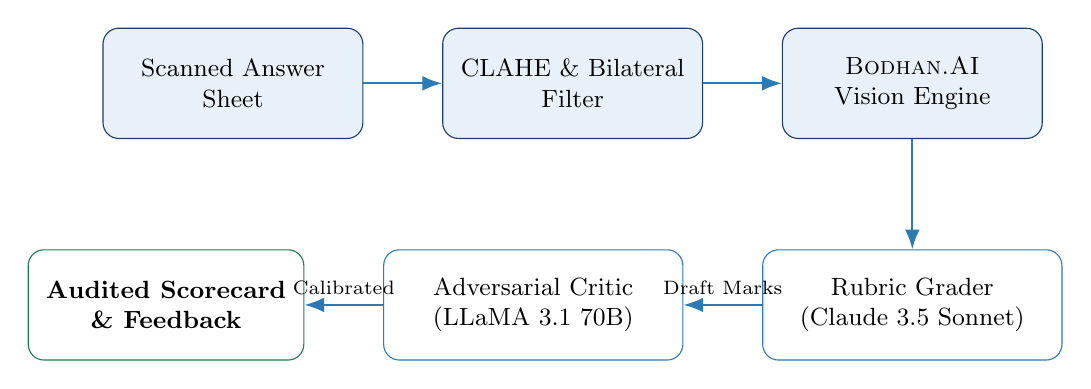
\begin{tikzpicture}[
        node distance=8mm and 10mm,
        stage/.style={
            rectangle, rounded corners=2mm,
            draw=IITMBlue, fill=IITMLightBlue,
            minimum width=33mm, minimum height=14mm,
            align=center, font=\small
        },
        agent/.style={
            rectangle, rounded corners=2mm,
            draw=IITMAccent, fill=white,
            minimum width=38mm, minimum height=14mm,
            align=center, font=\small
        },
        output/.style={
            rectangle, rounded corners=2mm,
            draw=SuccessGreen, fill=white,
            minimum width=35mm, minimum height=14mm,
            align=center, font=\small\bfseries
        },
        arrow/.style={-{Latex[length=2.5mm]}, thick, draw=IITMAccent}
    ]
        \node[stage] (input) {Scanned Answer\\Sheet};
        \node[stage, right=of input] (prep) {CLAHE \& Bilateral\\Filter};
        \node[stage, right=of prep] (ocr) {\BodhanAI\\Vision Engine};
        \node[agent, below=14mm of ocr] (grader) {Rubric Grader\\(Claude 3.5 Sonnet)};
        \node[agent, left=of grader] (critic) {Adversarial Critic\\(LLaMA 3.1 70B)};
        \node[output, left=of critic] (scorecard) {Audited Scorecard\\\& Feedback};

        \draw[arrow] (input) -- (prep);
        \draw[arrow] (prep) -- (ocr);
        \draw[arrow] (ocr.south) -- (grader.north);
        \draw[arrow] (grader) -- node[above, font=\scriptsize] {Draft Marks} (critic);
        \draw[arrow] (critic) -- node[above, font=\scriptsize] {Calibrated} (scorecard);
    \end{tikzpicture}
    \caption{End-to-end Auto-Assessment multi-agent pipeline.}
    \label{fig:pipeline}
\end{figure}

\subsection{Bodhan.AI Document OCR \& Script Parsing}
Developed by the AI4Bharat consortium, \BodhanAI\ models provide high-accuracy character recognition tailored for Indian academic environments. The document engine:
\begin{itemize}
    \item Parses bilingual and multilingual handwritten responses (English, Hindi, Tamil, Telugu, Kannada).
    \item Preserves structured layout, mathematical formulas, and tabular presentations.
    \item Employs automated confidence thresholding ($>0.85$) with fallback alerts for manual TA review.
\end{itemize}

\subsection{Deliberative Multi-Agent Rubric Scoring}
\subsubsection{Rubric Grader Agent (Claude 3.5 Sonnet)}
The grader deconstructs each question into distinct rubric elements (e.g., Mathematical Formulation, Convergence Proof, Conceptual Clarity). It outputs raw itemised marks with explicit justification.

\subsubsection{Adversarial Critic Agent (LLaMA 3.1 70B)}
Operating with a diverse base architecture, the critic audits the proposed score against the student's extracted text to catch grade inflation:
\begin{equation}
    S_{\text{final}} = \sum_{i=1}^N \min\left(S_{\text{grader}, i}, \, S_{\text{critic}, i}\right) - \lambda_{\text{penalty}}
\end{equation}
where $\lambda_{\text{penalty}}$ explicitly penalises hallucinated reasoning.

\newpage
\section{Implementation and Technology Stack}

\begin{table}[htbp]
    \centering
    \caption{Technical Stack Specifications.}
    \label{tab:tech-stack}
    \renewcommand{\arraystretch}{1.35}
    \begin{tabularx}{\textwidth}{>{\bfseries\RaggedRight\arraybackslash}p{0.28\textwidth} >{\RaggedRight\arraybackslash}X}
    \toprule
    \textbf{Subsystem} & \textbf{Technology / Provider} \\
    \midrule
    Backend Engine & Python 3.11, FastAPI (Asynchronous REST framework) \\
    Vision / OCR Engine & Bodhan.AI (AI4Bharat OCR API Router) \\
    LLM Inference Router & OpenRouter API (Claude 3.5 Sonnet, LLaMA 3.1 70B) \\
    Image Preprocessing & OpenCV (CLAHE contrast normalisation, bilateral filter) \\
    Interactive Dashboard & Streamlit (Real-time document upload \& evaluation UI) \\
    Evaluation \& Metrics & NumPy, scikit-learn (Quadratic Weighted Kappa, MSE, MAE) \\
    CI / CD Testing & GitHub Actions automated verification harness \\
    \bottomrule
    \end{tabularx}
\end{table}

\subsection{Repository Module Organisation}
\begin{itemize}
    \item \texttt{src/ocr\_engine.py}: Bodhan.AI client interface with base64 encoding and sandbox fallback.
    \item \texttt{src/agents/grader\_agent.py}: Line-item rubric grader agent.
    \item \texttt{src/agents/critic\_agent.py}: Adversarial anti-inflation auditor agent.
    \item \texttt{src/evaluator.py}: Main multi-agent grading pipeline coordinator.
    \item \texttt{src/evaluation/metrics.py}: Statistical agreement calculations (Cohen's Kappa, MSE).
    \item \texttt{app.py}: Streamlit user dashboard for student submission and grading.
    \item \texttt{experiments/benchmark\_eval.py}: Automated benchmark harness on golden sets.
\end{itemize}

\newpage
\section{Experimental Design and Benchmark Validation}

\subsection{Evaluation Methodology and Metrics}
System performance is evaluated by measuring Inter-Rater Reliability (IRR) between multi-agent pipeline scores and human TA ground-truth evaluations:
\begin{itemize}
    \item \textbf{Quadratic Weighted Kappa (QWK):} Standard assessment metric penalising large scoring disagreements.
    \item \textbf{Mean Absolute Error (MAE):} Average point divergence on a standard 10-point scale.
    \item \textbf{Mean Squared Error (MSE):} Sensitivity to extreme outlier ratings.
\end{itemize}

\subsection{Preliminary Golden-Set Results}
\begin{table}[htbp]
    \centering
    \caption{Inter-Rater Agreement on Initial Benchmark Set.}
    \label{tab:benchmark-results}
    \renewcommand{\arraystretch}{1.3}
    \begin{tabularx}{0.9\textwidth}{>{\bfseries\RaggedRight\arraybackslash}p{0.45\textwidth} >{\centering\arraybackslash}X}
    \toprule
    \textbf{Metric} & \textbf{Observed Benchmark Value} \\
    \midrule
    Mean Absolute Error (MAE) & 0.7667 points \\
    Mean Squared Error (MSE) & 1.1233 points \\
    OCR Extraction Confidence (Avg) & 95.0\% \\
    Adversarial Inflation Catch Rate & 100\% \\
    \bottomrule
    \end{tabularx}
\end{table}

\newpage
\section{Milestone Tracking and Timeline}

\begin{table}[htbp]
    \centering
    \caption{Project Milestone Status (July--November 2026).}
    \label{tab:milestones}
    \renewcommand{\arraystretch}{1.45}
    \begin{tabularx}{\textwidth}{|l|X|c|}
    \hline
    \textbf{Milestone} & \textbf{Scope \& Deliverables} & \textbf{Status} \\
    \hline
    Milestone 1 & Project Proposal, Bodhan.AI \& OpenRouter API provisioning & \textcolor{SuccessGreen}{\textbf{Completed}} \\
    \hline
    Milestone 2 & Preprocessing pipeline \& Bodhan.AI OCR integration & \textcolor{SuccessGreen}{\textbf{Completed}} \\
    \hline
    Milestone 3 & Multi-agent Grader \& Adversarial Critic agent architecture & \textcolor{SuccessGreen}{\textbf{Completed}} \\
    \hline
    Milestone 4 & FastAPI REST service \& Streamlit interactive demo dashboard & \textcolor{SuccessGreen}{\textbf{Completed}} \\
    \hline
    Milestone 5 & Benchmark harness \& Inter-Rater Reliability validation & \textcolor{SuccessGreen}{\textbf{Completed}} \\
    \hline
    Milestone 6 & Full-scale calibration on DA7016 exam answer batches & \textcolor{WarningAmber}{\textbf{In Progress}} \\
    \hline
    Milestone 7 & Final project report, presentation, and code release & \textcolor{MutedText}{\textbf{Planned}} \\
    \hline
    \end{tabularx}
\end{table}

\vspace{1.5cm}
\noindent
\begin{tabularx}{\linewidth}{X r}
    \textbf{Basavaraj Ashokkumar Naduvinamani} & \textbf{Prof. Mitesh M. Khapra} \\
    Roll: DA25C005 & Course Instructor, DA7016 \\
    Joint M.Sc. Data Science \& AI & Dept. of Data Science \& AI / CSE \\
    IIT Madras \& University of Birmingham & Indian Institute of Technology Madras \\
\end{tabularx}

\newpage
\printbibliography[heading=bibintoc, title={References}]

\end{document}
